\documentclass[11pt]{article}
% Кодировка и язык
\usepackage[utf8]{inputenc}           % Кодировка исходного файла (UTF-8)
\usepackage[T2A]{fontenc}             % Кодировка шрифтов для кириллицы
\usepackage[english,russian]{babel}   % Локализация: русские названия, переносы

% Поиск в PDF
\usepackage{cmap}                     

% Поля страницы
\usepackage{geometry}
\geometry{left=2cm, right=2cm, top=2cm, bottom=2cm}

% Математика
\usepackage{amsmath, amssymb, amsthm} % Базовые пакеты для математики
\usepackage{mathtools}                % Расширение amsmath (доп. символы и окружения)

% Картинки
\usepackage{graphicx}                 % Вставка картинок (\includegraphics)
\graphicspath{{pictures/}}            % Путь к папке с картинками
\usepackage{float}                    % Позволяет использовать [H] для жёсткого позиционирования
\usepackage{wrapfig}                  % Обтекание текста вокруг картинок

% Таблицы
\usepackage{array}                    % Расширенные возможности для таблиц
\usepackage{booktabs}                 % Красивые таблицы (\toprule, \midrule, \bottomrule)
\usepackage{multirow}                 % Объединение строк в таблицах
\usepackage{tabularx}                 % Таблицы с автоматической шириной колонок
\usepackage{ragged2e}                 % Улучшенное выравнивание (используется в tabularx)

% Списки
\usepackage{enumitem}                 % Гибкая настройка списков (itemize, enumerate)

% Колонтитулы
\usepackage{fancyhdr}                 

% Гиперссылки
\usepackage{xcolor}                   % Работа с цветами
\usepackage{hyperref}                 % Гиперссылки, оглавление, перекрёстные ссылки

% Умные ссылки
\usepackage{cleveref}                 

% Типографика
\usepackage{microtype}                % Улучшает переносы и межсловные расстояния

% Подписи к картинкам и таблицам
\usepackage{caption}                  % Настройка подписей (шрифт, отступы)

% Рисование схем и графиков
\usepackage{tikz}                     % Рисование схем, графиков, диаграмм
\usepackage{pgfplots}                 % Построение графиков функций (на основе tikz)
\pgfplotsset{compat=newest}           % Версия совместимости pgfplots

% Алгоритмы и код
\usepackage{algorithm}                % Окружения для алгоритмов
\usepackage{algorithmic}              % Синтаксис для алгоритмов
\usepackage{listings}                 % Вставка кода с подсветкой синтаксиса


% Настройка нумерации секций и подсекций
\renewcommand{\thesection}{\arabic{section}}                   
\renewcommand{\thesubsection}{\thesection.\arabic{subsection}} 


% Настройка списков: убираем лишние отступы слева
\setlist[itemize]{leftmargin=}
\setlist[enumerate]{leftmargin=}


% Определение окружений для теорем, лемм, определений и т.д.
% Нумерация привязана к номеру секции
\newtheorem{theorem}{Теорема}[section]
\newtheorem{definition}{Определение}[section]
\newtheorem{remark}{Замечание}[section]
\newtheorem{lemma}{Лемма}[section]
\newtheorem{example}{Пример}[section]
\newtheorem{consequence}{Следствие}[section]
\newtheorem{algorithmm}{Алгоритм}
\newtheorem{question}{Вопрос}[section]
\newtheorem{answer}{Ответ}[section]
\newtheorem{statement}{Утверждение}[section]


% Определение цветов
\definecolor{pblue}{rgb}{0.13,0.13,1}    
\definecolor{pgreen}{rgb}{0,0.5,0}       
\definecolor{pred}{rgb}{0.9,0,0}         
\definecolor{pgrey}{rgb}{0.46,0.45,0.48}

\newcommand{\lectureNumber}{10}
\newcommand{\lectureTitle}{Построение сигма-алгебры событий. Борелевские множества. Теорема Каратеодори. Мера Лебега}
\newcommand{\courseName}{Теория вероятностей}
\newcommand{\semester}{3 семестр, 2026/2027 уч. год}

\pagestyle{fancy}
\fancyhf{}
\fancyhead[L]{Ох, я такая скорая на помощь}
\fancyhead[R]{\thepage}
\setlength{\headheight}{15pt}

\hypersetup{
    colorlinks=true,
    linkcolor=blue!70!black,
    citecolor=blue!70!black,
    filecolor=blue!70!black,
    urlcolor=blue!70!black,
}

\begin{document}


\begin{titlepage}
    \centering
    
    {\large Московский физико-технический институт \par}
    {\large Высшая школа программной инженерии \par}
    \vspace{2cm}

    {\Large \textbf{\courseName} \par}
    {\large \semester \par}
    
    \vspace*{\fill}

    {\Huge \textbf{Лекция \lectureNumber} \par}
    {\Huge \textbf{\lectureTitle} \par}
    
    \vspace*{\fill}
    
    {\large Лектор: Широков Максим Евгеньевич  \par}
    {\large Автор: \href{https://t.me/mallina_olga}{Оля} \par}
\end{titlepage}

\pagenumbering{arabic}

\section{Построение сигма-алгебры событий}
\begin{definition}
    Вспомним, что тройка Колмогорова это $\{ \Omega, \mathcal{F}, \mathbb{P} \}$. 
    Здесь $\Omega$ --- произвольное множество, элементы которого мы считаем элементарными событиями (оно может быть счётным, а может быть и не счётным).
    Также выделенная нами сигма-алгебра $\mathcal{F}$ и  $\mathbb{P} : \mathcal{F} \to [0,1], \mathbb{P}$ --- вероятностная мера:
    \[ 1) \mathbb{P}(\varnothing) = 0, \ \mathbb{P}(\Omega) = 1  \]
    \[ 2) \mathbb{P} ( \bigcup_k A_k) = \sum_{k} P(A_k) \] 
\end{definition}

Теперь поговорим о следующих двух задачах:
\begin{enumerate}
    \item Как строить $\mathcal{F}$
    \item Как строить $\mathbb{P}$ (при заданной $\mathcal{F}$)
\end{enumerate}
Разберёмся с первой задачей, но сначала разберём следующую лемму:

\begin{lemma}
    Пусть $\Omega$ --- произвольное множество и $\mathcal{E}$ --- класс подмножеств в $\Omega$.\\
     Тогда $\exists! \sigma$-алгебра $\sigma(\mathcal{E})$ т.ч.:
     \begin{enumerate}
        \item $ \mathcal{E} \subseteq \sigma(\mathcal{E}) $
        \item Если $\mathcal{F}$ --- любая $\sigma$-алгебра т.ч. $\mathcal{E} \subseteqq \mathcal{F}$, то $\sigma(\mathcal{E}) \subseteq \mathcal{F}$
     \end{enumerate} 
\end{lemma}


\begin{example}
    Вспомним из "школьной" математики понятие выпуклой оболочки множества. Пусть у нас есть невыпуклое множество A. Мы знаем, что у каждого невыпуклого множества есть однозначно определённое множество, содержащее это невыпуклое. 
      \begin{figure}[H]
    \centering
    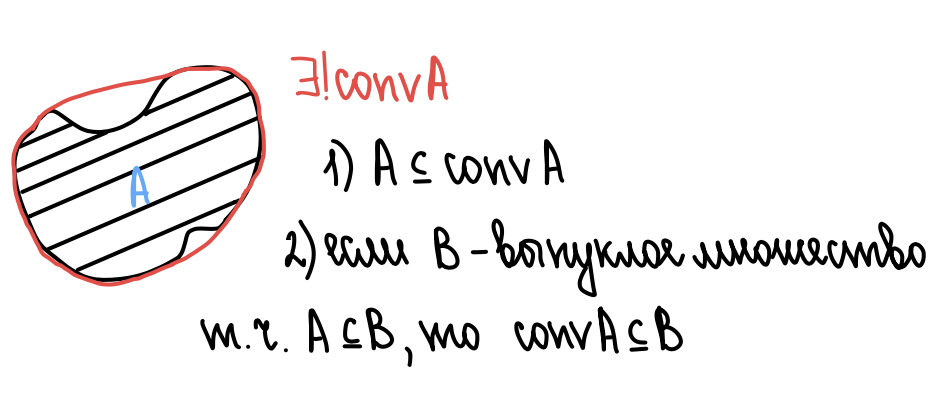
\includegraphics[width=0.65\linewidth]{примерчик для понимания.png}
\end{figure} 
\end{example}


\begin{example}
    Пусть $\mathcal{E} = \{A\}, \ A \subsetneq \Omega, \ A\neq \varnothing $. Тогда $\sigma(A) = \{ \varnothing, \Omega, A, \overline{A}$ \}. Фактически в этом примере $\sigma(A) = \sigma(\mathcal{E})$.
\end{example}

\begin{example}
    Пусть $\mathcal{E} = \{ A, B \}$. 
      \begin{figure}[H]
    \centering
    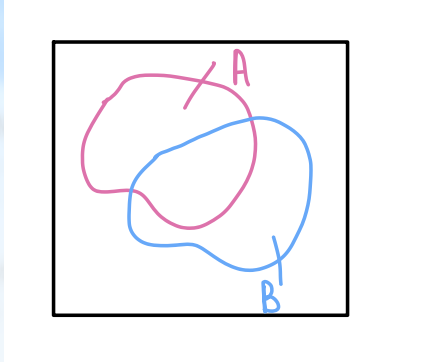
\includegraphics[width=0.5\linewidth]{картиночка для понимания.png}
\end{figure} 

    Имеем 4 множества: нештрихованное, штрихованное только розовым, штрихованное только голубым, штрихованное и розовым, и голубым. Обозначим их $D_1, D_2, D_3, D_4$. Оставим в качестве упражнения умному читателю проверить, что $\sigma(\mathcal{E}) = \{ \varnothing, D_1, ... , D_4, D_1D_2, ... , D_1D_2D_3 \Omega \} $. 
\end{example}


\begin{remark}
    На нашу лемму можно посмотреть следующим образом: 
      \begin{figure}[H]
    \centering
    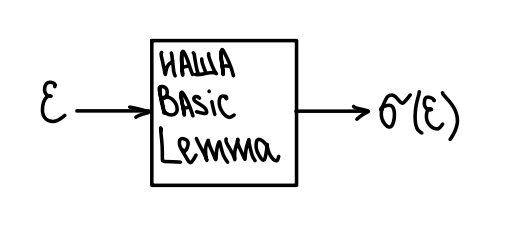
\includegraphics[width=0.65\linewidth]{basic lemma.png}
\end{figure} 
\end{remark}


\section{Борелевские множества}

\begin{definition}
    Борелевские множества строятся следующим образом: пусть $\Omega = [0,1]$. В качестве $\mathcal{E} = \{ [a,b] \subseteq \Omega \} (a\leq b)$. 
    Тогда $\sigma(\mathcal{E}) := B([0,1])$ --- борелевская $\sigma$-алгебра в отрезке $[0,1]$. \\
    Поймём, что за объект мы получили. Имеем:
    \begin{itemize}
        \item $[a,b] \in B([0,1])$
        \item $(a,b) \in B([0,1])$. Поймём, почему это так:
        $(a,b) =  [a,b] \setminus (\{a\}, \{b\}) $\\
        Также имеем, так как в этом классе содержатся интервалы, то и полуинтервалы тоже:
        \item $ (a,b] \in B([0,1])$
        \item $[a,b) \in B([0,1])$ \\
        Также заметим, что 
        \item $Q\in B([0,1])$ (здесь $Q$ --- множество рациональных точек)
        \item $I\in B([0,1])$ (здесь $I$ --- множество иррациональных точек)
    \end{itemize}
\end{definition}

\begin{definition}
    Борелевскую $\sigma$-алгебру можно определить как минимальную $\sigma$-алгебру, содержащую открытые подмножества. То есть, действительно, альтернативный способ: 
    \[ \mathcal{E}' = \{ (a,b) \} \]  
      \begin{figure}[H]
    \centering
    \includegraphics[width=0.5\linewidth]{еще одна картиночка с леммой.png}
\end{figure} 
    Также можно взять следующий затравочный класс:
    \[ \mathcal{E}'' = \{ [a,b) \} \]
\end{definition}

\begin{definition}
    Определим борелевскую $\sigma$-алгебру в $\mathbb{R}^n$ : $B(\mathbb{R}^n)$ 
    \[ \mathcal{E} = \{ \text{все открытые шары} \} \] 
    Напомним, что шар это:
    \[ U _{\varepsilon, r} = \{ \overline{x} \in \mathbb{R}^n | \rho (\overline{x},\overline{r}) < \varepsilon \} \]
\end{definition}

Теперь разберёмся со следующим вопросом: как строить $\mathbb{P}$. Здесь на помощь нам придёт теорема Каратеодори.

\begin{theorem}
    (Каратеодори) Пусть $\mathcal{E}_0$ --- алгебра подмножеств в $\Omega$ и $\mathbb{P}_0$ --- конечно-аддитивная мера на $\mathcal{E}_0$ т.ч. $\mathbb{P}_0(\varnothing) = 0, \mathbb{P}_0(\Omega) = 1$.
    Конечная аддитивность означает, что 
    \[ \mathbb{P}_0 (\displaystyle \bigcup_{i=1}^n A_i) = \sum _{i=1}^n \mathbb{P}_0 (A_i), A_i \cap A_j =\varnothing \ \forall i,j \]
    Также потребуем, чтобы эта функция $\mathbb{P}_0$ была непрерывна в 0, то есть:
    \[ \forall A_n\supseteq A_{n+1} \supseteq A_{n+2} \supseteq \ldots : \bigcap_{k=1}^\infty A_k = \varnothing, \ A_k\in \mathcal{E}_0 \ \forall k \]
    \[ \lim\limits_{k\to \infty} \mathbb{P}_0(A_k) = 0 \] 
    Тогда $\exists!$ счётно-аддитивная вероятностная мера $\mathbb{P}$ на $\sigma(\mathcal{E}_0) = F$ т.ч. сужение этой счётно-аддитивной меры совпадает с $\mathbb{P}_0$: $| \mathbb{P}|_{\mathcal{E}_0} = \mathbb{P}_0$. 
\end{theorem}


\section{Мера Лебега}

\begin{definition}
    $\Omega = [0,1], \mathcal{E}_0 = \{$алгебра, порождённая отрезками $[a,b]$ и интервалами $(a,b) \}$. Тогда $\mathbb{P}_0 (A) = l(A)$.
    В данном случае $\sigma(\mathcal{E}_0) = B([0,1])$. 
\end{definition}











\end{document}